\subsection{Memory}
Below we report on the results we have for measuring RAM access time and RAM bandwidth.

\subsubsection{RAM access time}
Results from the memory latency benchmark are
plotted as a series of data sets as shown in Figure ~\ref{fig:f1}.
Each data set represents a stride size, with the array
size varying from 4KB up to 16MB. The
curves contain a series of horizontal plateaus, where
each plateau represents a level in the memory hierarchy. The point where each plateau ends and the line
rises marks the end of that portion of the memory hierarchy.\\
\\
The sizes of L1, L2, L3 cache observed here are 32K, 256K, 4M respectively.
The observed L1 and L2 cache sizes match that of our expectation.
However, we only observed a L3 cache of 4MB instead of 8MB.
Our hypothesis is that
only part of the L3 cache is assigned to one core in a multi-core scenario.

\begin{figure}[htb]
    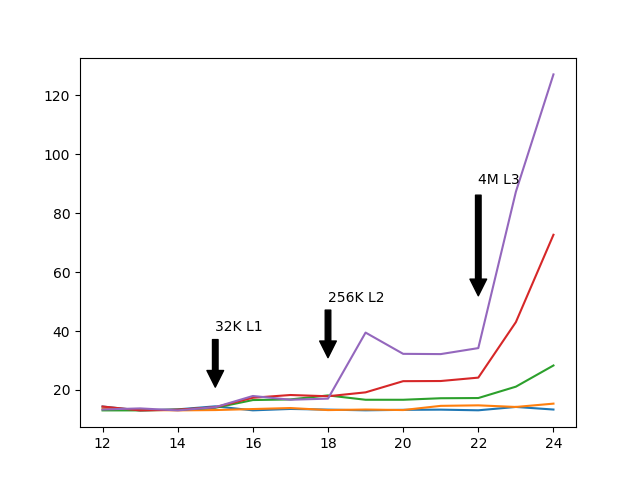
\includegraphics[width=8cm]{fig1_latency.png}
    \centering
    \caption{Memory latency}
    \label{fig:f1}
\end{figure}

\subsubsection{RAM bandwidth}
The mean, min and max values of average read/write speed for ten rounds are reported in Table ~\ref{tab:t6}. 
We noticed that we did not observe the ideal memory bandwidth (25 GB/s) in case.
There are many possible factors. 
One is that we could have measurement errors. 
The other is that we have extra operations in both experiments.
Even though the read/write time should dominate the time,
they still play a minor role.

\begin{table}[H]
\caption{Mean, min and max values of average read/write speed for ten runs}
\begin{tabular}{|c|c|c|c|c|} 
    \hline
    Type & Mean (GB/s) & Min (GB/s)& Max (GB/s)& Stddev\\ 
    \hline
    Read & 16.275760& 16.179897 & 16.359991 & 0.057545\\
    \hline
    Write & 13.406692 & 13.326650 & 13.465415 & 0.049811\\ 
    \hline
   \end{tabular}
    \label{tab:t6}
\end{table}

\subsubsection{Page fault service time}
Since we don't have a filesystem, this measurement is skipped.